\documentclass[11pt]{article}
\usepackage{graphicx}
\usepackage{fullpage}
\usepackage{fourier}
\usepackage{xspace}
\usepackage{booktabs}
\usepackage{wrapfig}
\begin{document}
\title {cse13s asgn1 WRITEUP.pdf}
\author{Lucas Lee; CruzID: luclee}
\date {1/11/2022}
\maketitle
\section{Program Analysis}\label{ss:analysis}
When this program runs, it creates temporary files that store the data needed to make the different collatz sequence graphs. These plots are printed when plot.sh is finished running, unless the xdg-open \textless example.pdf \textgreater does not work on your computer (on my windows computer the open command does not work and this was the only way for me to open pdf files in my virtual machine).

\section{Graphs, Bash Commands, Program comments}\label{ss:misc}
\begin{figure}[h]
\begin{centering}
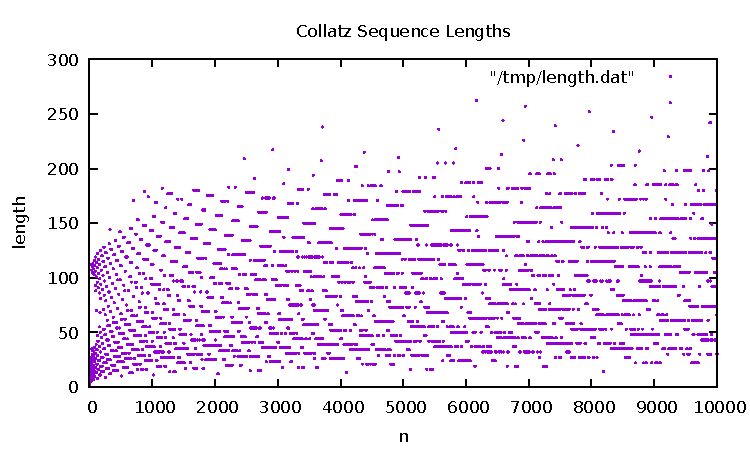
\includegraphics[width=0.75\textwidth]{fig/length.pdf}
\caption{Collatz Sequence Length Graph}\label{fig:1}
\end{centering}
\end{figure}

\begin{figure}[h]
\begin{centering}
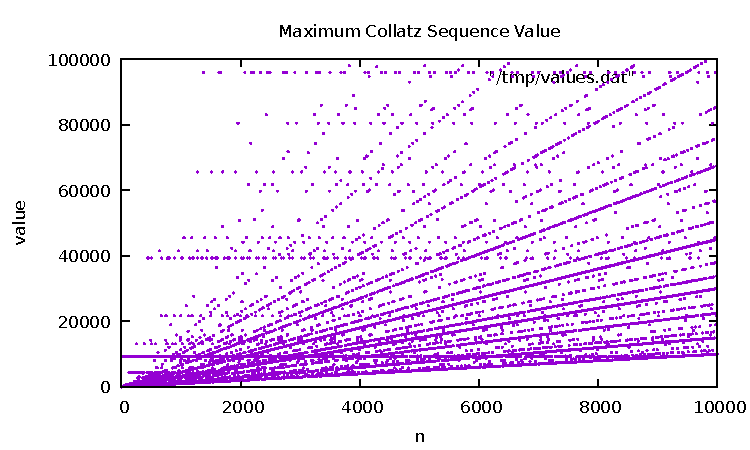
\includegraphics[width=0.75\textwidth]{fig/values.pdf}
\caption{Collatz Sequence Maximum Values Graph}\label{fig:2}
\end{centering}
\end{figure}

\begin{figure}[h]
\begin{centering}
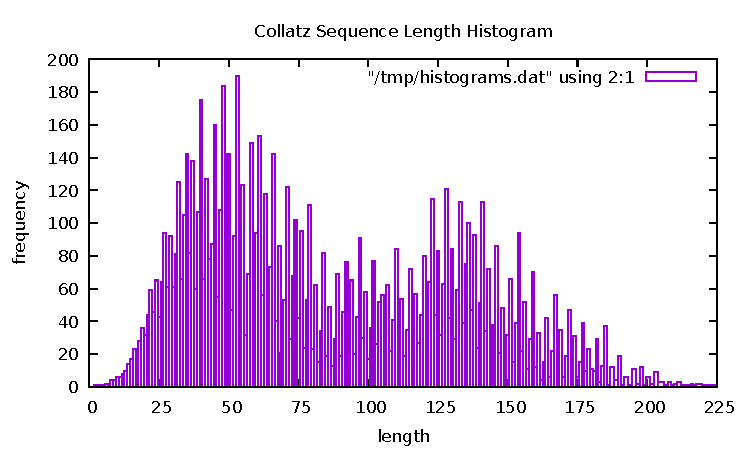
\includegraphics[width=0.75\textwidth]{fig/histogram.pdf}
\caption{Collatz Sequence Length Histogram Graph}\label{fig:3}
\end{centering}
\end{figure}

For my Collatz sequence length graph, I used the wc -l command, to get the number of lines in each run of the Collatz sequence. In order to format my file correctly for gnuplot to plot my file, I put an echo -n command to numerically track the length of each time I ran the Collatz sequence in my for loop. My program had spacing problems when I used the echo command, so I had to add space after my echo command in order to correctly format the data file for gnuplot to read.\\
For my Collatz sequence maximum values graph, I used the sort and head commands connected with pipes. I used the sort -nr command to sort the Collatz values from greatest to least, and used the head -n 1 command to get the first value after it sorts from greatest to least. After it does this, it prints to the temporary file. I thought using these commands would be the best possible way to get a max value since it is easy to sort a file of numbers numerically and take the max.\\
For my Collatz sequence histogram, I used the sort -n command combined with the uniq -c command. I used to sort -n command to clump all of the similar lengthed Collatz sequences and followed it with the uniq -c command to give me a two columned data file that had the frequency of similar length sequences in the first column, and the length of each sequence in the second column. I had trouble using gnuplot's histogram command, since the plot histogram command reads 1 column of data, so I decided to use boxes and use the 2:1 command in my plot line to flip the way gnuplot reads my columns. In order for me to get my axis labels correct, I had to manually type out the x and y ranges, as well as using xtics and ytics to get specific intervals on my axis labels.\\
I took a lot of inspiration from Eugene's examples and explanations in his lab section. I had a lot of trouble following along, since I have a windows computer and my commands are a bit different. For example, I had to look up commands to open pdf files in my virtual machine because I could not open them with a ssh connection to my local machine. I had to use the xdg-open command in my code to open the pdf files in my virtual machine, so I am not sure if this works the same for mac terminals, but the open command does not work for my computer.
\end{document}

